% Options for packages loaded elsewhere
\PassOptionsToPackage{unicode}{hyperref}
\PassOptionsToPackage{hyphens}{url}
%
\documentclass[
]{article}
\usepackage{amsmath,amssymb}
\usepackage{lmodern}
\usepackage{iftex}
\ifPDFTeX
  \usepackage[T1]{fontenc}
  \usepackage[utf8]{inputenc}
  \usepackage{textcomp} % provide euro and other symbols
\else % if luatex or xetex
  \usepackage{unicode-math}
  \defaultfontfeatures{Scale=MatchLowercase}
  \defaultfontfeatures[\rmfamily]{Ligatures=TeX,Scale=1}
\fi
% Use upquote if available, for straight quotes in verbatim environments
\IfFileExists{upquote.sty}{\usepackage{upquote}}{}
\IfFileExists{microtype.sty}{% use microtype if available
  \usepackage[]{microtype}
  \UseMicrotypeSet[protrusion]{basicmath} % disable protrusion for tt fonts
}{}
\makeatletter
\@ifundefined{KOMAClassName}{% if non-KOMA class
  \IfFileExists{parskip.sty}{%
    \usepackage{parskip}
  }{% else
    \setlength{\parindent}{0pt}
    \setlength{\parskip}{6pt plus 2pt minus 1pt}}
}{% if KOMA class
  \KOMAoptions{parskip=half}}
\makeatother
\usepackage{xcolor}
\usepackage[margin=1in]{geometry}
\usepackage{graphicx}
\makeatletter
\def\maxwidth{\ifdim\Gin@nat@width>\linewidth\linewidth\else\Gin@nat@width\fi}
\def\maxheight{\ifdim\Gin@nat@height>\textheight\textheight\else\Gin@nat@height\fi}
\makeatother
% Scale images if necessary, so that they will not overflow the page
% margins by default, and it is still possible to overwrite the defaults
% using explicit options in \includegraphics[width, height, ...]{}
\setkeys{Gin}{width=\maxwidth,height=\maxheight,keepaspectratio}
% Set default figure placement to htbp
\makeatletter
\def\fps@figure{htbp}
\makeatother
\setlength{\emergencystretch}{3em} % prevent overfull lines
\providecommand{\tightlist}{%
  \setlength{\itemsep}{0pt}\setlength{\parskip}{0pt}}
\setcounter{secnumdepth}{-\maxdimen} % remove section numbering
\ifLuaTeX
  \usepackage{selnolig}  % disable illegal ligatures
\fi
\IfFileExists{bookmark.sty}{\usepackage{bookmark}}{\usepackage{hyperref}}
\IfFileExists{xurl.sty}{\usepackage{xurl}}{} % add URL line breaks if available
\urlstyle{same} % disable monospaced font for URLs
\hypersetup{
  pdftitle={Final Project },
  pdfauthor={Imanbayeva Sofya, Mazzi Lapo, Piras Mattia, Srivastava Dev },
  hidelinks,
  pdfcreator={LaTeX via pandoc}}

\title{Final Project \vspace{1in}}
\usepackage{etoolbox}
\makeatletter
\providecommand{\subtitle}[1]{% add subtitle to \maketitle
  \apptocmd{\@title}{\par {\large #1 \par}}{}{}
}
\makeatother
\subtitle{Group 22 \vspace{1in}}
\author{Imanbayeva Sofya, Mazzi Lapo, Piras Mattia, Srivastava Dev
\vspace{1in}}
\date{May 2023 \vspace{1in}}

\begin{document}
\maketitle

\newpage

\newpage

\hypertarget{question-1}{%
\section{Question 1}\label{question-1}}

We have chosen Station 55 for our analysis.

We will first present some time series plots to understand the data
observed. After that we will fit a Gaussian HMM model and use it to
interpret the first question of interest.

\hypertarget{data-visualization}{%
\section{Data Visualization}\label{data-visualization}}

\begin{center}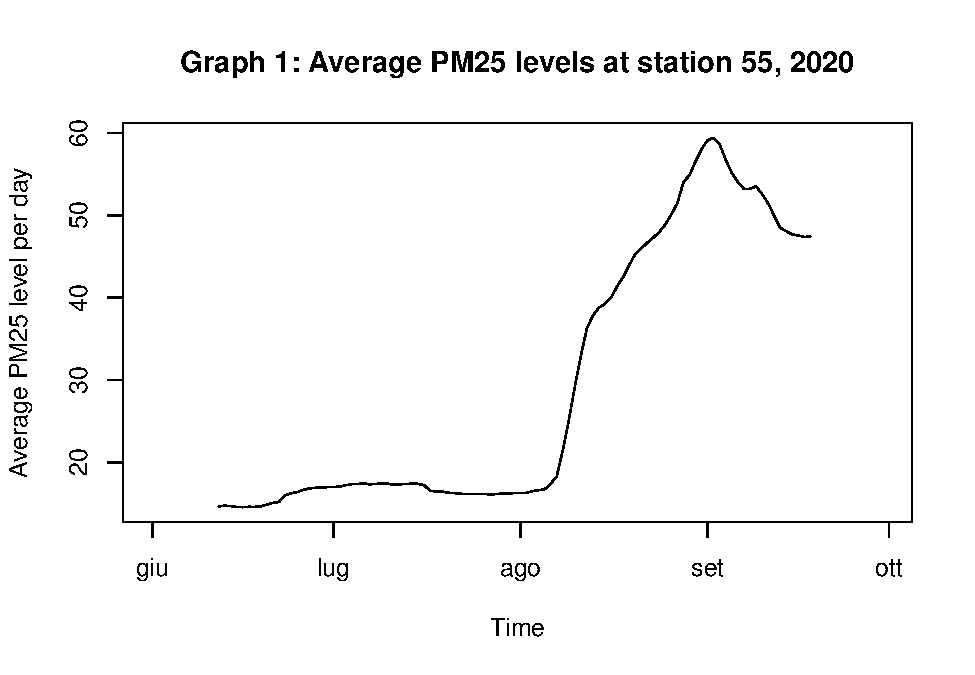
\includegraphics[width=0.75\linewidth,height=0.75\textheight]{finalproject_files/figure-latex/time series pm25-1} \end{center}

Moving average dramatically increases in the beginning of August from
around 17 to its peak in the beginning of September at around 60 in its
PM25 levels. The values slightly decrease in September.

\begin{center}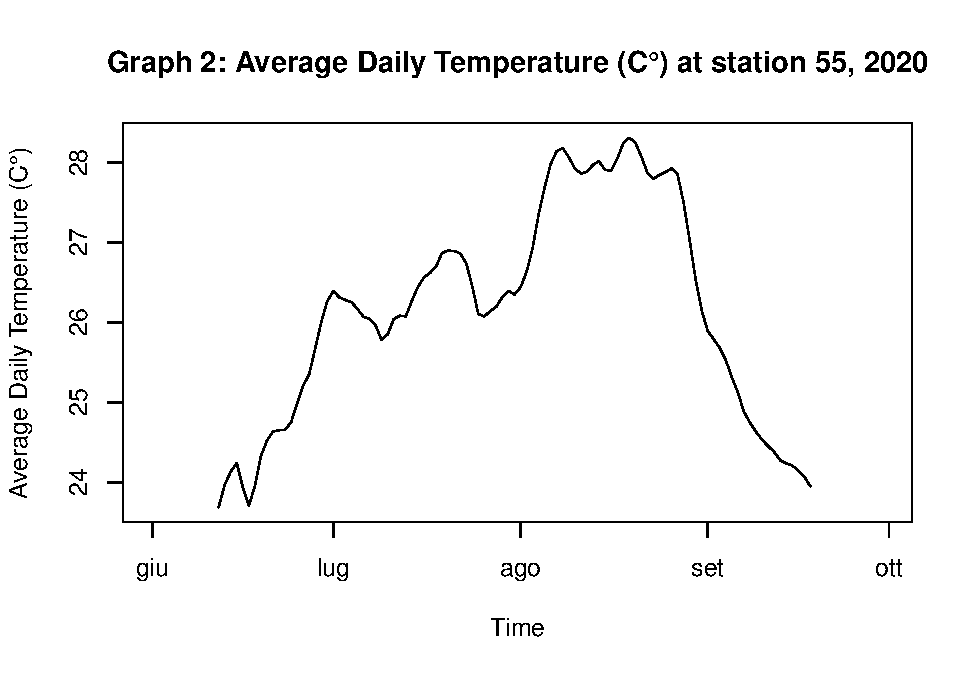
\includegraphics[width=0.75\linewidth,height=0.75\textheight]{finalproject_files/figure-latex/ts temp-1} \end{center}

The temperature has been increasing from June's values of 24 degrees
Celsius to its peak in August at around 28.

\begin{center}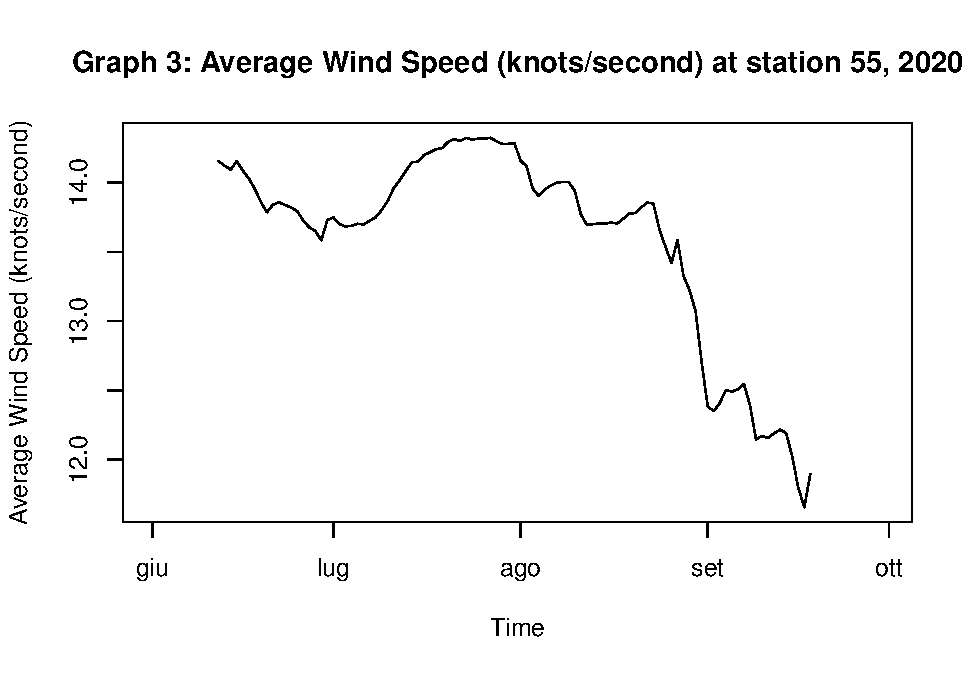
\includegraphics[width=0.75\linewidth,height=0.75\textheight]{finalproject_files/figure-latex/ts wind-1} \end{center}

Average wind level has been stable at around 14m/s in the summer and
started to decrease in the second part of August to around 12 in
mid-September.

\begin{center}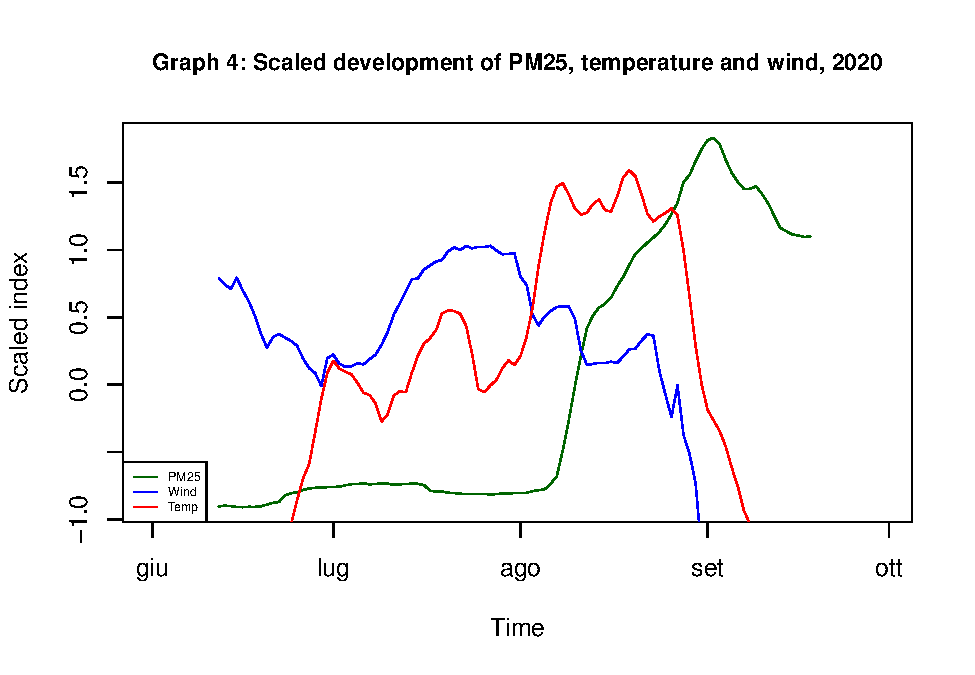
\includegraphics[width=0.75\linewidth,height=0.75\textheight]{finalproject_files/figure-latex/compare-1} \end{center}

High average temperature in August and comparatively strong winds seem
to have a correlation with fires, which have increased the values of
PM25 particles in the air. There is around 10 day lag between the
temperature increases and PM25 value increase in August.

\begin{center}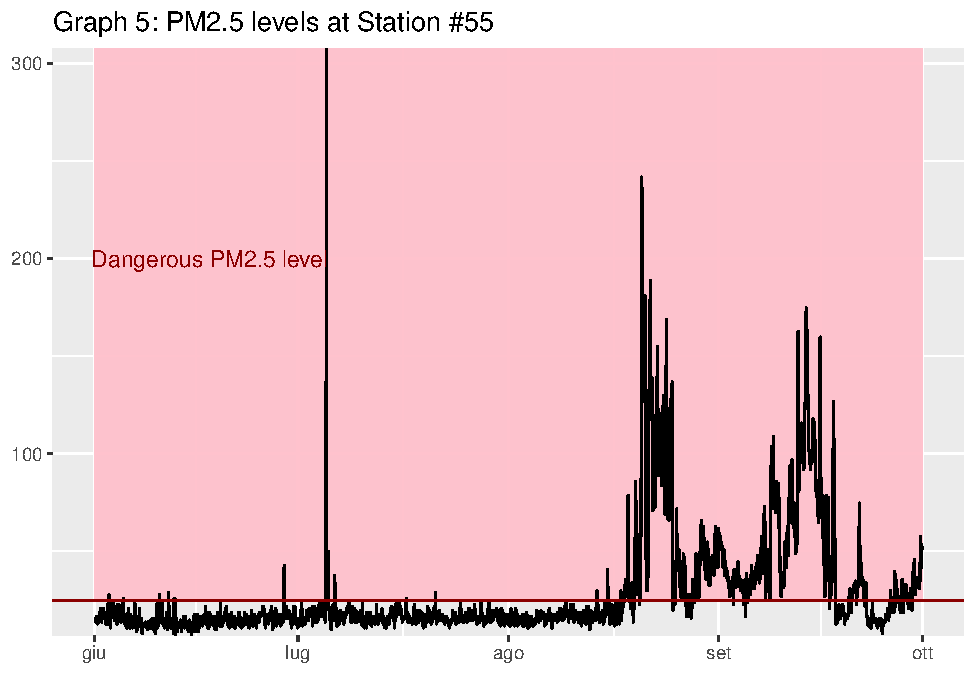
\includegraphics[width=0.75\linewidth,height=0.75\textheight]{finalproject_files/figure-latex/PM25 levels-1} \end{center}

Majority of measurements from June to mid-August are smaller than the
prescribed limit with the exception of a peak of an outlying 307.81 in
July. However, since then until October, the dynamic has changed with
only a few days where the values staying within the limit constraints
below 25. The peaks are high, probably resulted from fires, high
temperatures and strong wind.

\begin{center}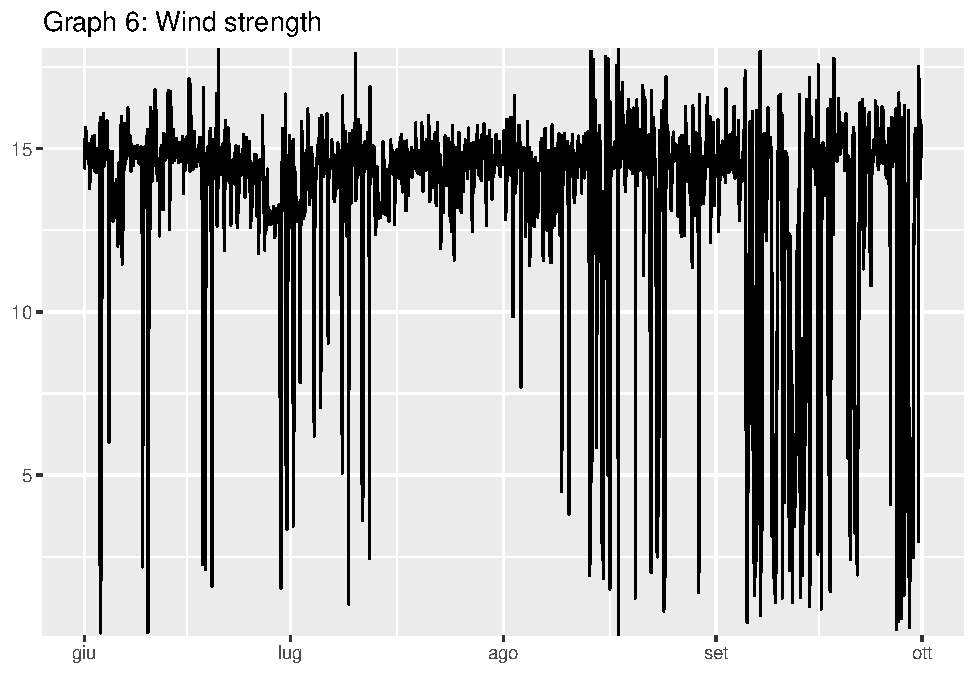
\includegraphics[width=0.75\linewidth,height=0.75\textheight]{finalproject_files/figure-latex/wind levels-1} \end{center}

\hypertarget{gaussian-hmm-model}{%
\section{Gaussian HMM Model}\label{gaussian-hmm-model}}

\begin{equation*}
\begin{cases}
Y_t = \mu_1 + \epsilon_t, \quad \epsilon_t \overset{iid}{\sim} N(0, \sigma_1^2)  
& \text{if the state $S_t=1$} \\
Y_t = \mu_2 + \epsilon_t, \quad \epsilon_t \overset{iid}{\sim} N(0, \sigma_2^2) 
&\text{if the state $S_t=2$}. \\

Y_t = \mu_3 + \epsilon_t, \quad \epsilon_t \overset{iid}{\sim} N(0, \sigma_3^2) 
& \text{if the state $S_t=3$} \\

\end{cases}
\end{equation*} First, we set up our model. The initial probabilities
and the transition matrix are just made by default values. Since, there
are 3 states, they will have 1/3 probability each. {[}

\begin{tabular}{c|ccc}
State & 1 & 2 & 3 \\
\hline
Probability & $\pi_1$ & $\pi_2$ & $\pi_3$
\end{tabular}
\begin{pmatrix}
p_0(1) = \frac{1}{3}\\

p_0(2) = \frac{1}{3} \\

p_0(3) = \frac{1}{3}
\end{pmatrix}

{]}

\begin{verbatim}
## Initial state probabilities model 
##   pr1   pr2   pr3 
## 0.333 0.333 0.333 
## 
## Transition matrix 
##         toS1  toS2  toS3
## fromS1 0.333 0.333 0.333
## fromS2 0.333 0.333 0.333
## fromS3 0.333 0.333 0.333
## 
## Response parameters 
## Resp 1 : gaussian 
##     Re1.(Intercept) Re1.sd
## St1               0      1
## St2               0      1
## St3               0      1
\end{verbatim}

The results of the estimation of both the initial probabilities and the
transition matrix are indicated below.

\begin{verbatim}
## converged at iteration 23 with logLik: -9089.537
\end{verbatim}

\begin{verbatim}
## Initial state probabilities model 
## pr1 pr2 pr3 
##   1   0   0 
## 
## Transition matrix 
##         toS1  toS2  toS3
## fromS1 0.993 0.007 0.000
## fromS2 0.023 0.951 0.026
## fromS3 0.000 0.043 0.957
## 
## Response parameters 
## Resp 1 : gaussian 
##     Re1.(Intercept) Re1.sd
## St1          15.891  3.005
## St2          33.303  8.086
## St3          91.324 36.054
\end{verbatim}

Firstly, we can identify the three states that we wanted to study. State
1 is the one relative to low pollution, state 3 is relative to high
pollution levels and state 2 is the one that we can associate to a
medium pollution levels. Looking at the transition matrix we note that
there are steps that are never possible, state 3 to 1 and vice versa.

Further, the states are very persistent, and probability of state
transition by a single step is very low, and by two steps virtually
zero. Thus, the current state is a very good predictor of the state in
the next hour.

If the current state is of low pollution, there is not much need to
enforce any strict measures, with an extremely high probability (0.993)
of staying the same low pollution state.

If the current state is of medium pollution, there is a need to enforce
strict measures for some time, given the large probability of staying in
the medium state (0.95), and also a possibility of transitioning to high
pollution state in the next hour(0.026).

Finally, if the pollution is high prolonged strict measures should be
anticipated to bring it down medium pollution and finally to low
pollution (prolonged because) both high and medium pollution states
being highly persistent.

The following table gives the expected number of hours for pollution
state to move from i to j (where i and j are different).

\begin{verbatim}
##             low    medium     high
## low     0.00000 136.52717 280.8998
## medium 69.18944   0.00000 152.9230
## high   92.61855  23.42911   0.0000
\end{verbatim}

Thus we can see that if the current state is of high pollution, it'll
take an expected time of 92 hours for the pollution to reach the low
pollution state and 23 hours to reach the medium pollution state. Again
given the persistence of each state, the first passage time is a good
metric for predicting outcomes over the next hours.

Finally, below is the prediction of the states, given the data observed.

\begin{center}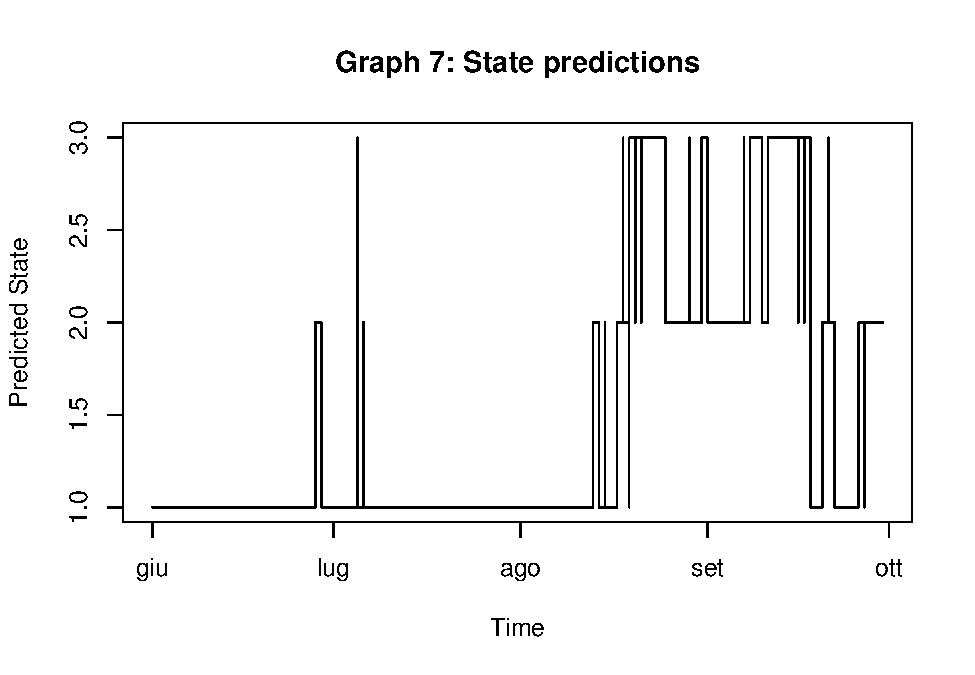
\includegraphics[width=1\linewidth,height=0.75\textheight]{finalproject_files/figure-latex/unnamed-chunk-2-1} \end{center}

\hypertarget{question-2}{%
\section{Question 2}\label{question-2}}

For our analysis we decided to use stations 55, 92, 97 and 41.

\begin{center}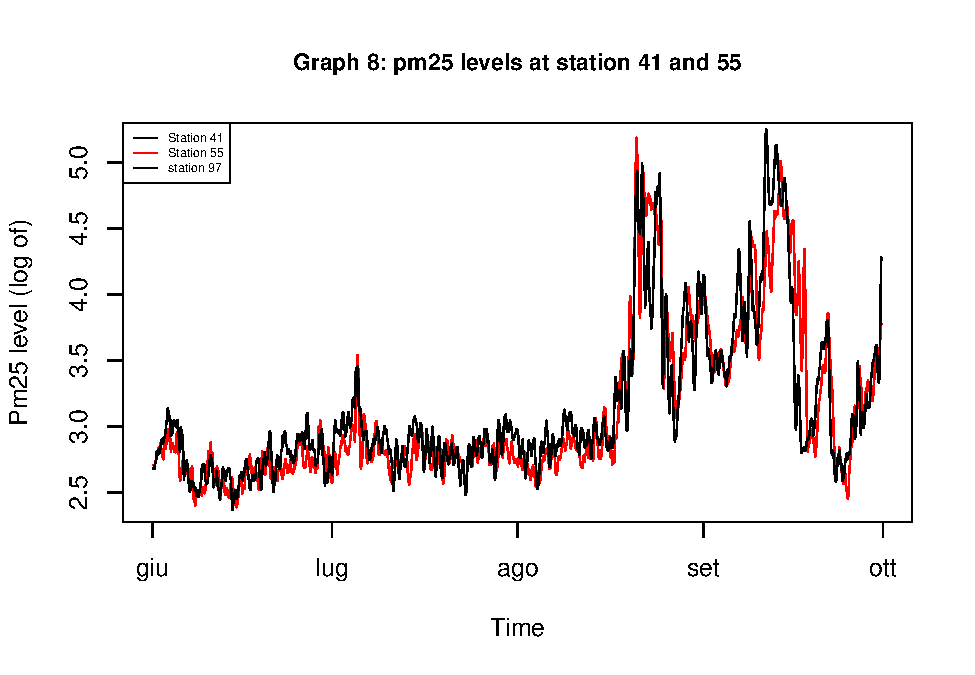
\includegraphics[width=0.75\linewidth,height=0.75\textheight]{finalproject_files/figure-latex/Graph 8-1} \end{center}

\begin{center}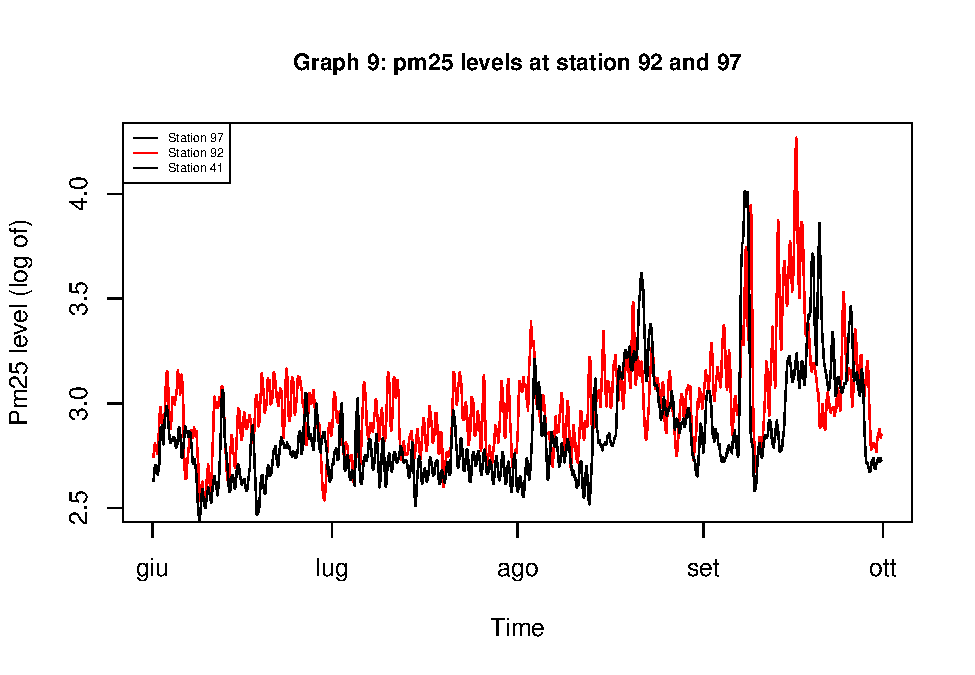
\includegraphics[width=0.75\linewidth,height=0.75\textheight]{finalproject_files/figure-latex/Graph 9-1} \end{center}

\begin{center}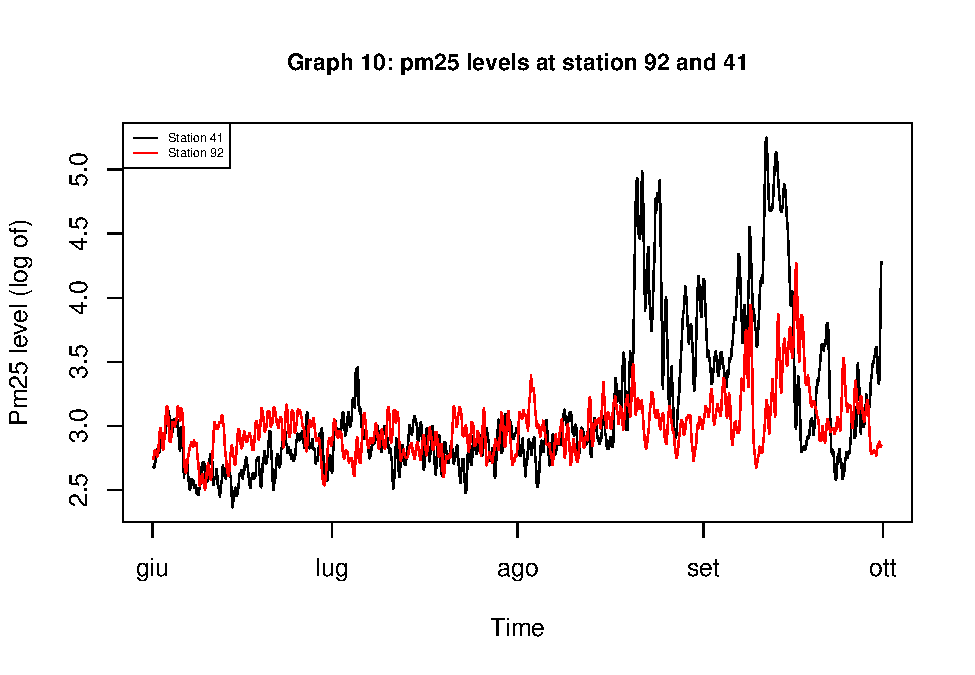
\includegraphics[width=0.75\linewidth,height=0.75\textheight]{finalproject_files/figure-latex/Graph 10-1} \end{center}

In case of spatial dependence we expect the graphs of the closer
stations to be more aligned compared to the ones which are more distant.
Stations 55 and 41 are the closest one (only 100km apart) and we can see
from Graph 8 that their measurement of pm25 almost coincide, supporting
the spatial dependency hypothesis. Stations 92 and 97 are almost 300 km
apart, and we can see from Graph 9 that their overlap is lower compared
to the previous figure. This is even more clear if we look at Graph 10.
Stations 41 and 92 are the furthest apart (650 km) and we can see that
their observations are the less synchronized, especially in the Autumn
months. Thus we can affirm from this rough first analysis that there is
the case for a phenomenon of spatial dependence.

\hypertarget{model-specification}{%
\section{Model specification}\label{model-specification}}

To set up a model that accounts for the spatial dependency we first need
a formula to calculate the distance between stations. We decided to use
the geometrical based on the coordinates of the stations.

\[
distance_{i,j} = \sqrt{{(long_{i}-long_{j} )^2 + (lat_{i}-lat_{j})^2}}
\]

\end{document}
